\documentclass[runningheads]{llncs}
\usepackage{graphicx}

\begin{document}

\title{Weather trend prediction and forecasting based on synthetical methods of regression and DNN}
\author{Muhan Hu\inst{1} \and Han Weng\inst{1} \and Fangrui Zhu\inst{1}}

\institute{Electrical and Computer Engineering, University Of Waterloo, 200 University Avenue W, Waterloo, ON, Canada, N2L 3G1. \\ \bfseries Authors in alphabetical order by last name.}

\maketitle 

\begin{abstract}
    This is a project aiming at predicting weather based on some historical weather data from two perspectives. First, time-series regression models were used to predict the trend of a specific value in a given period, in order to give people an idea of how temperature, pressure will change in a city of interest in the next few years. The second part is about forecasting weather condition days later with given features including temperature, pressure and humidity. This is a classification problem and in particular we use a deep neural network (DNN) model.
    
    \keywords{Weather forecasting \and Time-series regression \and DNN.}
\end{abstract}

%%%%%%%%%%%% Section %%%%%%%%%%%%%%
\section{Introduction}
Within centuries weather forecasting has been a topic given much attention to by meteorologist. Conventional weather prediction was based on direct meteorological observation, for example cloud movement from satellites and other profession apparatus. Nowadays, with the rise of data science, predicting weather solely with easily measured data like temperature, humidity has more and more being an emphasis. A number of modern machine learning approaches have been applied to this old subject, including ARIMA (Auto-Regressive Integrated Moving Average), ANN (Artificial Neural Network)\cite{abrahamsen2018machine,holmstrom2016machine} and DNN (Deep Neural Network)\cite{liu2014deep}. Our goal is to a) give a prediction and visualization of how temperature, humidity and pressure will change in the next following years based on periodic historical data, and b) make weather condition forecasting based on given features mentioned above.

Unlike the forecasting part which is simple DNN classification application, the first task is more challenging and less straightforward, therefore additional literature research was done in the first place. It is obvious that a successful time series forecasting depends on an appropriate model fitting. A lot of efforts have been done by researchers over many years for the development of efficient models to improve the forecasting accuracy. As a result, various important time series forecasting models have been evolved in literature. One of the most popular and frequently used stochastic time series models is the Autoregressive Integrated Moving Average (ARIMA) model. The basic assumption made to implement this model is that the considered time series is linear and follows a particular known statistical distribution, such as the normal distribution. ARIMA model has subclasses of other models, such as the Autoregressive (AR), Moving Average (MA) and Autoregressive Moving Average (ARMA) models. \cite{arxivadhi}

There are also other complicated models for time series. Box and Jenkins\cite{boxcali} had proposed a quite successful variation of ARIMA model, the Seasonal ARIMA (SARIMA). Peter Zhang \cite{zhangneur} also discussed artificial neural networks (ANNs) model for time series analysis. However, the popularity of the ARIMA model is mainly due to its flexibility to represent several varieties of time series with simplicity. Therefore we decided to choose this straight-forward and popular ARIMA model.


%%%%%%%%%%%% Section %%%%%%%%%%%%%%
\section{Dataset preparation}
\subsection{Dataset description}
There are 5 raw dataset contains hourly data for 30 cities during 6 years for these features:
\begin{itemize}
	\item temperature
	\item pressure
	\item humidity
    \item wind direction 
    \item wind speed
	\item weather condition
\end{itemize}

\begin{figure}
    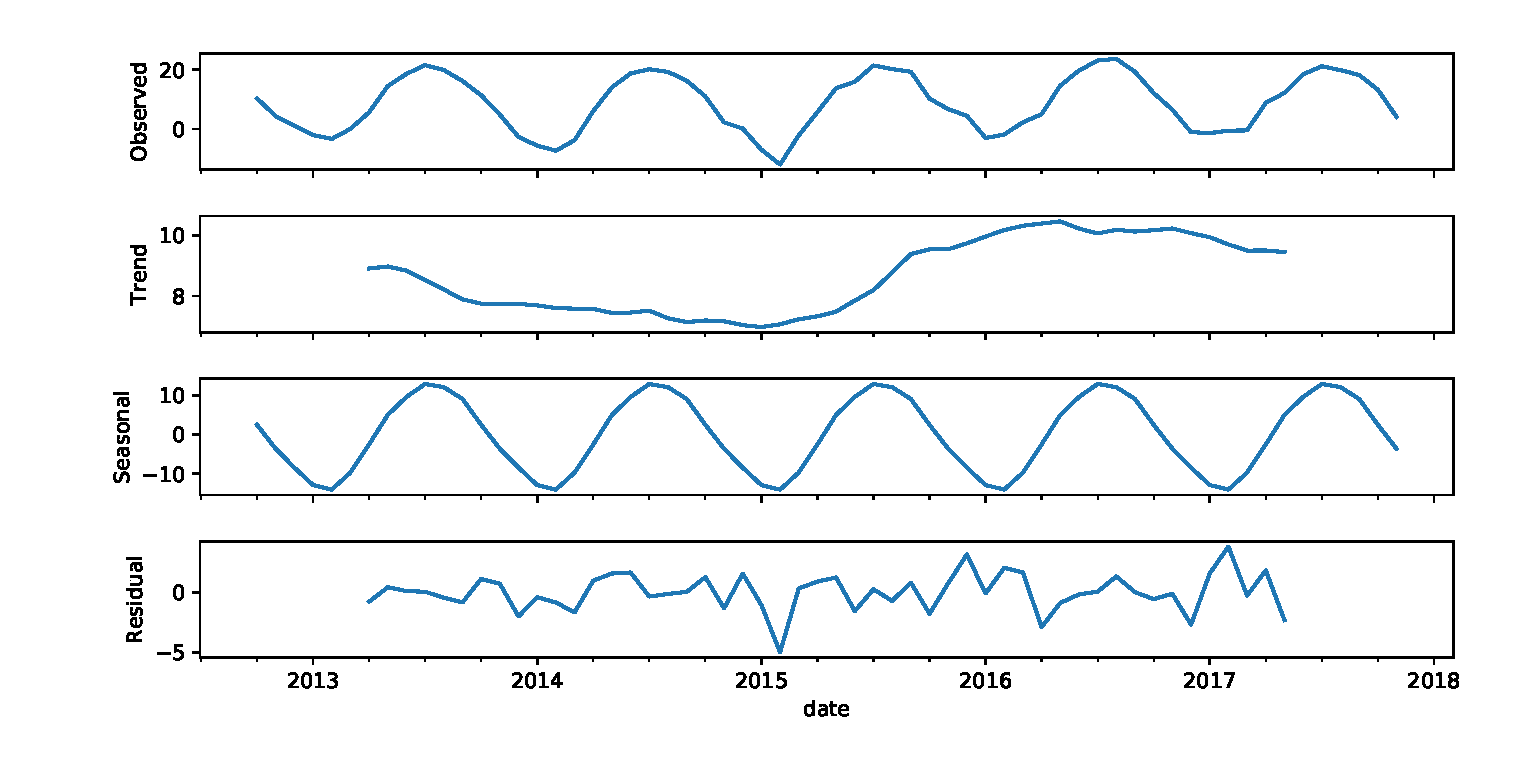
\includegraphics[width=\textwidth]{Toronto-decomposition.eps}
    \caption{Decomposed time series (Toronto monthly temperature from 2012-2017)}\label{toronto-decomp}
\end{figure}

\subsection{Transform dataset to be ready for machine learning}
Since reading the whole dataset into python is slow, unnecessary and not scalable, we used Apache Spark, a distributed computing system to preprocess data. Also, the dataset contains missing fields and have some inconsistency in formats and categories, therefore data cleaning and filtering are performed in this stage as well. We finally got two machine-learning-ready datasets for later work:

\subsubsection{Dataset for trend prediction}
Command line arguments are passed to the spark program to determine which city, which feature is chosen and whether monthly or daily data is required. Finally the datasets generated are time series data in following format:
(timestamp, value\_of\_selected\_feature) for a chosen city.

\subsubsection{Dataset for weather forecasting}
Again, command line arguments are passed to the spark program to determine which city is studied. The spark program automatically gathers data from different raw datasets matching the timestamp. Finally training (classification) dataset is generated as follows: (date, hour, temperature, humidity, pressure, wind speed, weather condition). The four meteorological data are input features and the weather condition are labels. Originally there were 35 weather condition classes but finally the spark program provided an argument to combine some of them to give 13. This will be talked about in more details in the experiment part.

%%%%%%%%%%%% Section %%%%%%%%%%%%%%
\section{Part I - Trend prediction: the time series model}

\subsection{Stationarity check}

\begin{figure}
    \includegraphics[width=\textwidth]{Toronto-ACF.pdf}
    \caption{ACF plot}\label{toronto-acf}
\end{figure}

\begin{figure}
    \includegraphics[width=\textwidth]{Toronto-PACF.pdf}
    \caption{PACF plot}\label{toronto-pacf}
\end{figure}

Time series data consist of real valued measurements of multiple parameters at equal intervals. Time series prediction tasks assume that future values in the series are a function of historical values of the same series.

Before applying any statistical model on a time series, the series has to be stationary. A stationary time series is one whose statistical properties such as mean, variance, autocorrelation, etc. are all constant over time. Most statistical forecasting methods are based on the assumption that the time series can be rendered approximately stationary through the use of mathematical transformations. A stationarized series is relatively easy to predict and to be able to obtain meaningful sample statistics such as means, variances, and correlations with other variables. Such statistics are useful as descriptors of future behavior only if the series is stationary. 

We first check if our time series is stationary. The ADCF Test - Augmented Dickey–Fuller test is used to gives us various values that can help in identifying stationarity. The null hypothesis is that the time series is non-stationary. It comprises of a test statistics and some critical values for some confidence levels. If the test statistics is less than the critical values, we can reject the null hypothesis and say that the series is stationary. The ADCF test also gives us a p-value accuracy to the null hypothesis, the lower p-value we have, the better result we got.

Then we use decomposition function to decompose the time series data. This function has four components, trend (upward \& downward movement of the data with time over a large period of time), seasonality (seasonal variances), noise or irregularity (spikes and troughs at random intervals) and cyclicity (behavior that repeats itself after large interval of time, like months, years, etc.), these components can be used to do forecasting, prediction or extrapolation of missing data.

From Fig.~\ref{toronto-decomp}, we can see that trend and seasonality are two reasons why the time series is not stationary and hence need to be corrected. If the series has a long-run trend and tends to revert to the trend line following a disturbance, it may be possible to stationarize it by de-trending (e.g., by fitting a trend line and subtracting it out prior to fitting a model, or else by including the time index as an independent variable in a regression or ARIMA model), perhaps in conjunction with logging or deflating. For our Time Series, we use differencing to remove the trend, and use rolling window to remove the seasonality. Since the seasonality is yearly for our Time Series, we use w=12 as rolling statistics parameter here, which means choose 12 months as a cycle. For simplicity, we do logarithmic scale first because we can revert back to the original scale during forecasting. Since the temperature has negative values, we add 100 on every data point to make them all positive, then start data preprocessing.

We choose log scale transformation and time shift transformation to deal with the trend and compare which one is better based on ADCF test result. Log scale transformation use log scaled data minus moving average to smooth data. Time shift transformation use log scaled data minus shifted log scaled data to calculate the differencing. The ADCF test result of these two methods is shown in Table~\ref{adcfResults}. From Table~\ref{adcfResults}, we observe that p-value of log scale transformation has reduced compared to original value, but still larger than 0.05. However, p-value of time shift transformation is small enough to reject null hypothesis. Thus, time series after time shift transformation is ready for modeling.

\begin{table}
\caption{ADCF results of original time series and transformed time series.}\label{adcfResults}
\begin{tabular}{l|l|l|l}
\hline
Dickey Fuller Test Result & Original & Log Transformation & Time Shift Transformation\\
\hline
Test Statistic&	-0.800512&	-1.254808&	-8.879796\\
\hline
p-value	&0.818972&	0.649586&	1.3275E-14\\
\hline
\#Lags Used&	10	&10&	9\\
\hline
Observations Used	&51	&40&	51\\
\hline
Critical Value (1\%)&	-3.565624&	-3.605565&	-3.565624\\
\hline
Critical Value (5\%)&	-2.920142&	-2.937069&	-2.920142\\
\hline
Critical Value (10\%)&	-2.598015&	-2.606986&	-2.598015\\
\hline
\end{tabular}
\end{table}

\subsection{Regression}

A popular and widely used statistical method for time series forecasting is the ARIMA model. ARIMA is an acronym that stands for Auto-Regressive Integrated Moving Average. It is a generalization of the simpler Auto-Regressive Moving Average and adds the notion of integration. A nonseasonal ARIMA model is classified as an "ARIMA(p,d,q)" model, where p is the number of autoregressive terms, d is the number of nonseasonal differences needed for stationarity, and q is the number of lagged forecast errors in the prediction equation. For our case, d=1 because we did time shift transformation during preprocessing, and we need to use ACF and PACF plot to get p and q values.

ACF plot is Autocorrelation Function plot, autocorrelation refers to how correlated a time series is with its past values whereas the ACF is the plot used to see the correlation between the points, up to and including the lag unit. In ACF, the correlation coefficient is in the x-axis whereas the number of lags is shown in the y-axis. PACF plot is Partial Autocorrelation Function plot, which is a summary of the relationship between an observation in a time series with observations at prior time steps with the relationships of intervening observations removed. The partial autocorrelation at lag k is the correlation that results after removing the effect of any correlations due to the terms at shorter lags.

From Fig.~\ref{toronto-acf} and Fig.~\ref{toronto-pacf}, we can see that ACF is geometric, so q=0, and PACF is significant in the first and second lags, so p=2. However, the value for parameters (2,1,0) might not be our final choice, we’ll try more similar match including (2,1,1), (1,1,1), etc. to find out which one is the best.

We use AR, MA and ARIMA model to fit the data, and compare these three models to find the best one to do the prediction. A pure Auto Regressive (AR only) model is one where Yt depends only on its own lags, and a pure Moving Average (MA only) model is one where Yt depends only on the lagged forecast errors. After several tries, we use AR (2,1,0), MA (0,1,2) and ARIMA (2,1,2) to plot the data and fitted values. We use RSS value to compare these models, from Fig.~\ref{toronto-ar,toronto-ma,toronto-arima}, we can see that by combining AR and MA into ARIMA, RSS value has decreased, indicating ARIMA to be better than its individual component models.

\begin{figure}
    \centering
    \includegraphics[height=2.5in]{Toronto-MAmodel.eps}
    \caption{MA model plot with RSS value}\label{toronto-ma}
\end{figure}

\begin{figure}
    \centering
    \includegraphics[height=2.5in]{Toronto-ARmodel.eps}
    \caption{AR model plot with RSS value}\label{toronto-ar}
\end{figure}

\begin{figure}
    \centering
    \includegraphics[height=2.5in]{Toronto-ARIMAmodel.eps}
    \caption{ARIMA model plot with RSS value}\label{toronto-arima}
\end{figure}

With the ARIMA model built, we will now generate predictions. But, before we do any plots for predictions, we need to reconvert the predictions back to original form. This is because, our model was built on log transformed data. We add cumulative sum back to fitted values and calculate the exponential value, then minus 100 to get reconverted data.

\begin{figure}
    \centering
    \includegraphics[height=2.5in]{Toronto-pred.pdf}
    \caption{Predicted future trend of Toronto temperature}\label{toronto-pred}
\end{figure}

\subsection{Results}

Based on the ARIMA model, the prediction plot is shown as Fig.~\ref{toronto-pred}. The value on y-axis is still transformed data, but after we reconverted them, the predicted value and true value is compared in Table~\ref{toronto-pred-compare}. From Table~\ref{toronto-pred-compare}, we can see that predicted values and true values are close to each other, which means our model has good accuracy.

\begin{table}
    \centering
    \caption{Comparison between actual data and predicted data of Toronto temperature}\label{toronto-pred-compare}
    \begin{tabular}{l|l|l}
    \hline
    Date&	Actual Data&	Predicted Data\\ \hline
    2017-07-01&	21.106953&	22.40426\\ \hline
    2017-08-01&	19.825096&	21.353791\\ \hline
    2017-09-01&	18.181847&	17.158485\\ \hline
    2017-10-01&	13.234041&	11.012681\\ \hline
    2017-11-01&	4.049218&	4.47109\\ \hline
    \end{tabular}
\end{table}

Similarly, we did modeling and prediction for other cities. For Montreal, we compared AR (2,1,0), MA (0,1,2) and ARIMA (2,1,2), we finally choose ARIMA model because of lowest RSS value. (See Fig.~\ref{montreal-chicago-pred})

\begin{figure}
    \centering
    \includegraphics[width=2.3in]{Montreal-pred.pdf}
    \includegraphics[width=2.3in]{Chicago-pred.pdf}
    \caption{Predicted future trend. Left: Montreal. Right: Chicago}\label{montreal-chicago-pred}
\end{figure}

We use ARIMA (2,1,3) model for Chicago, and we use AR (4,1,0) model for Boston. (See Fig.~\ref{montreal-chicago-pred} and Fig.\ref{boston-pred})

\begin{figure}
    \centering
    \includegraphics[height=2.5in]{Boston-pred.pdf}
    \caption{Predicted future trend of Boston temperature}\label{boston-pred}
\end{figure}

From above results, it can be seen that the best models applied in each city are different, and not every city is suitable for ARIMA models. For example, AR model has better performance on Boston temperature data. The difference is that when we use the AR model or the MA model, the prediction interval is wider than the ARIMA model, which means there is more uncertainty associated with the forecast.

In summary, we use the ARIMA model to predict future temperature trend, which is limited to short-term predictions. It can be seen from the wide confidence interval in the prediction plots that the accuracy of the model cannot be guaranteed over long time. On the one hand, our data size is not big enough. We use the monthly data of 2012-2017 to build models, there are 5 cycles before and after, while the ideal data size should have more cycles (such as more than 20 years historical data) as training set, which can help us build more accurate models. On the other hand, our model is still not complicated enough. We just use the classical ARIMA model. Classical ARIMA models are typically well-suited for short-term forecasts, but not for longer term forecasts due to the convergence of the autoregressive part of the model to the mean of the time series. In addition, more complex models such as the seasonal ARIMA model can be used to do more research.

%%%%%%%%%%%% Section %%%%%%%%%%%%%%
\section{Part II - Weather forecasting: DNN classification}

\subsection{Data split}
The output data from Spark is very well organized and therefore ready to be studied. The dataset is split into three parts, including training dataset, test dataset and validation data set, which are used to train model, do prediction and test accuracy/loss in every epochs, respectively. The labels are shifted by 5 days using the timestamp column, therefore the features (i.e. humidity, wind speed, pressure, temperature) are measured 5 days before weather label and we are able to predict the weather condition five days later.

\begin{figure}
    \centering
    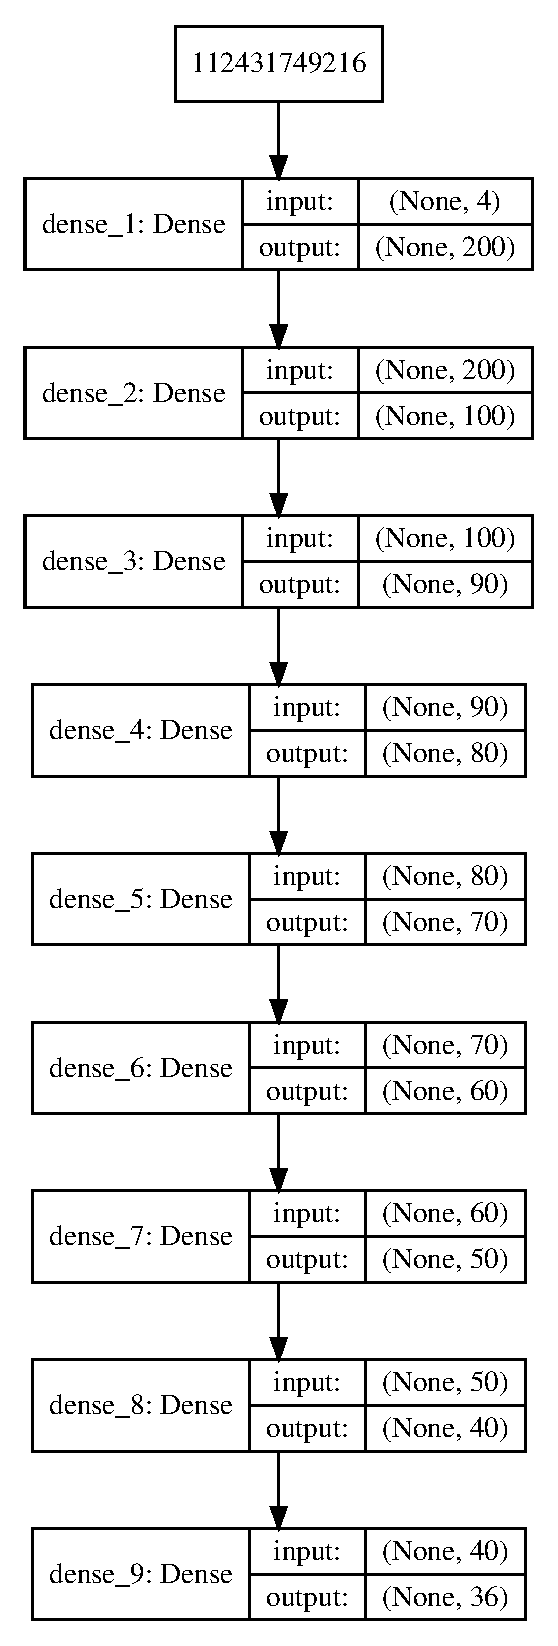
\includegraphics[height=5in]{model.eps}
    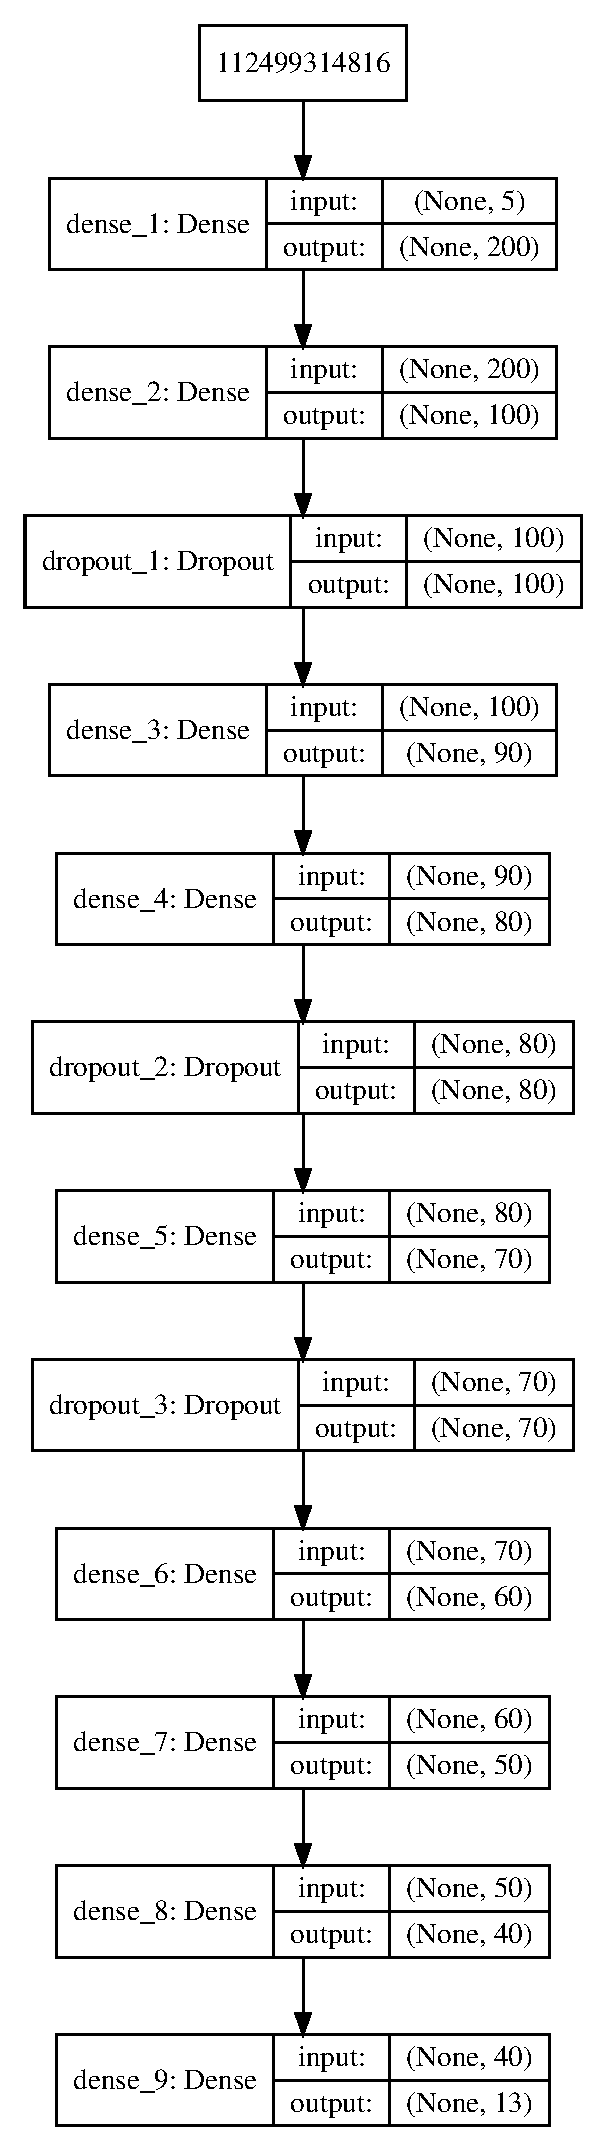
\includegraphics[height=5in]{model-with-drop.eps}
    \caption{Left: Initial DNN model setup. Right: DNN model setup with dropout layers added to deal with overfitting}\label{model}
\end{figure}

\subsection{Model construction}

The original model is constructed as Fig.~\ref{model} (left). It is a network with 7 hidden layers connecting I/O layers. We trained 10 models for 10 different cities using the network introduced above to start with, and got highest prediction accuracy at 60\% for Phoenix and 30\% as lowest in Vancouver from these initial experiments. Other cities' model had an accuracy ranging between these two. Since the process of trainings are identical for all cities, we will use the result for these two cities for further discussion in this report as they are typical for comparison.


\subsection{Combining label classes}
Original results are not satisfactory enough. One important reason we notice is that the weather labels in the raw data are too detailed and the information (4 features) we have may not be sufficient to predict the detailed weather. For example, ``broken clouds'' and ``few clouds'' may not have much difference in terms of temperature, humidity, wind and pressure. We therefore turned back to Spark and combined some very-closely-related labels into one label, making the number of classes decrease from 35 to 13. This gives the accuracies in most cities a 10\% to 30\% increase including Vancouver where the former model performed worst, while the performance in Phoenix almost remains the same. (Fig. ~\ref{cities})

\begin{figure}
    \centering
    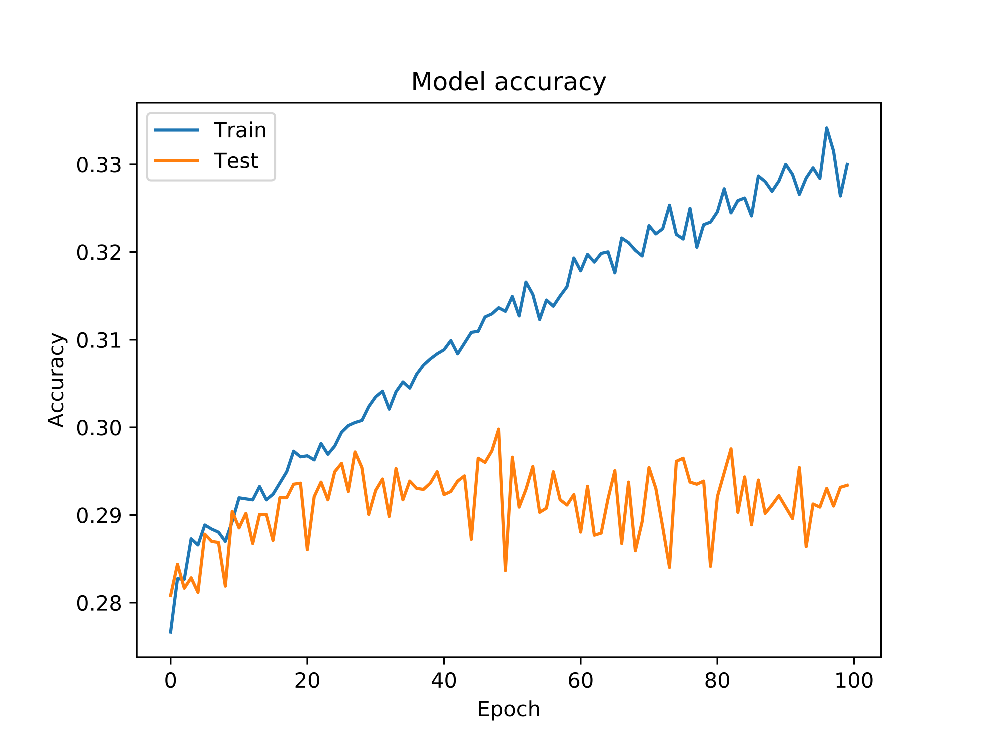
\includegraphics[width=2.3in]{vancouver-overfitting.eps}
    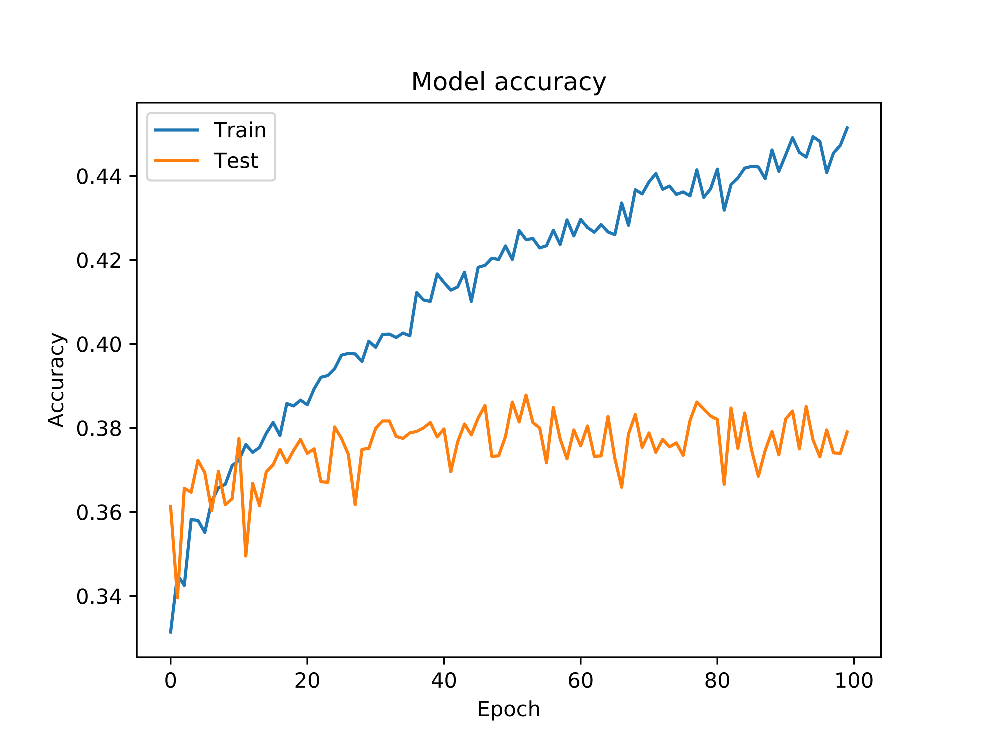
\includegraphics[width=2.3in]{vancouver-overfitting-after.eps}
    \caption{Accuracy of prediction in Vancouver. Left: using 35-class labels. Right: using 13-class labels.} \label{combine-label}
\end{figure}


\subsection{Dealing with overfitting}

The first-stage result is shown as Fig.~\ref{overfit}. The performance on the training set in Vancouver grows rapidly with epoch number but that for test set basically remains the same. Significant difference between the two lines can be observed as the epoch increases, which indicates severe overfitting. It is even more obvious when compared with the model in Phoenix.

We take a normal practice to solve this problem by adding dropout layers. The final DNN model is shown in Fig.~\ref{model} (right), with additional layers added after layer 2, 4 and 5. Exactly same experiment was performed on the Vancouver dataset and the results is shown in Fig.~\ref{van-final}.

\begin{figure}
    \centering
    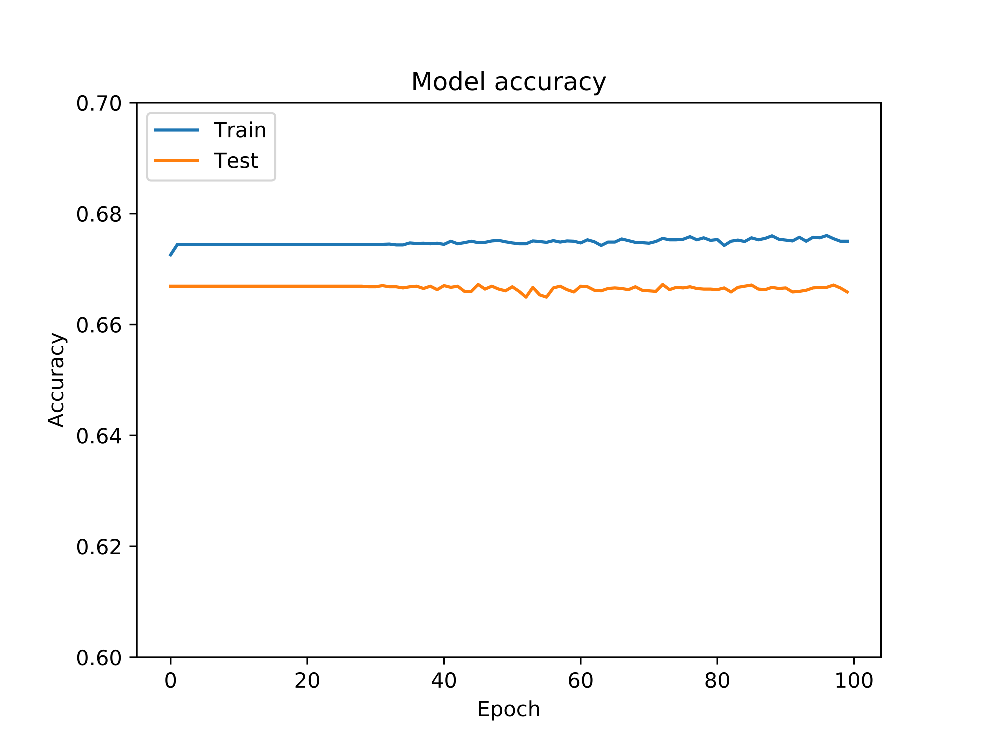
\includegraphics[width=2.3in]{phoenix-overfitting.eps}
    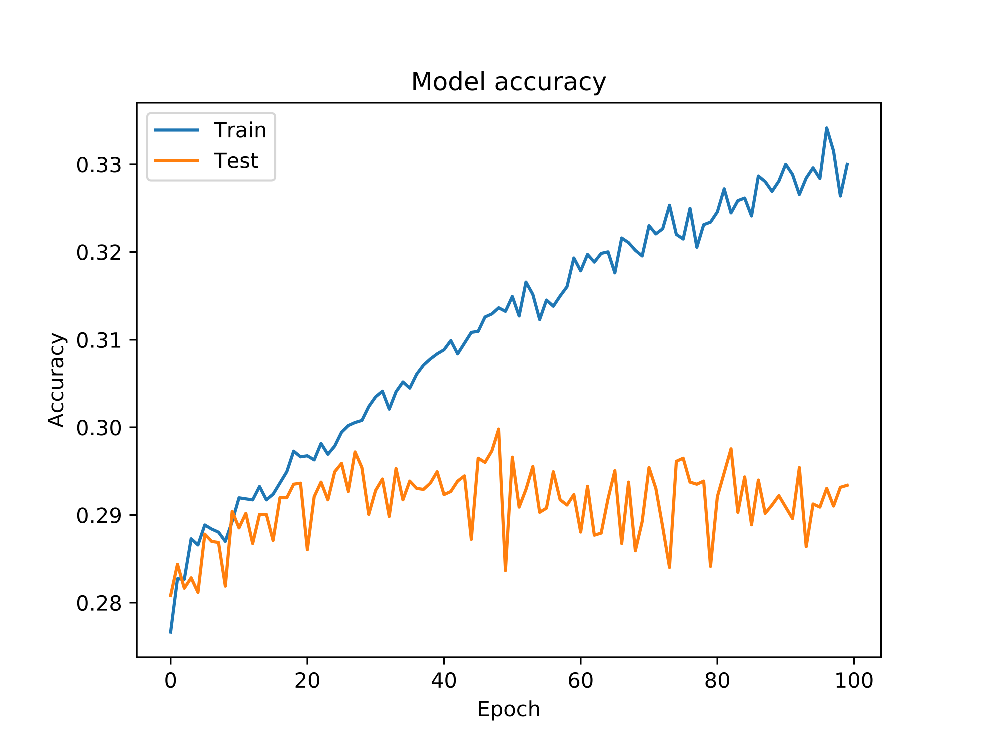
\includegraphics[width=2.3in]{vancouver-overfitting.eps}
    \caption{Classification accuracy after epochs illustrating overfitting problem. Left: Phoenix. Right: Vancouver}\label{overfit}
\end{figure}

\begin{figure}
    \centering
    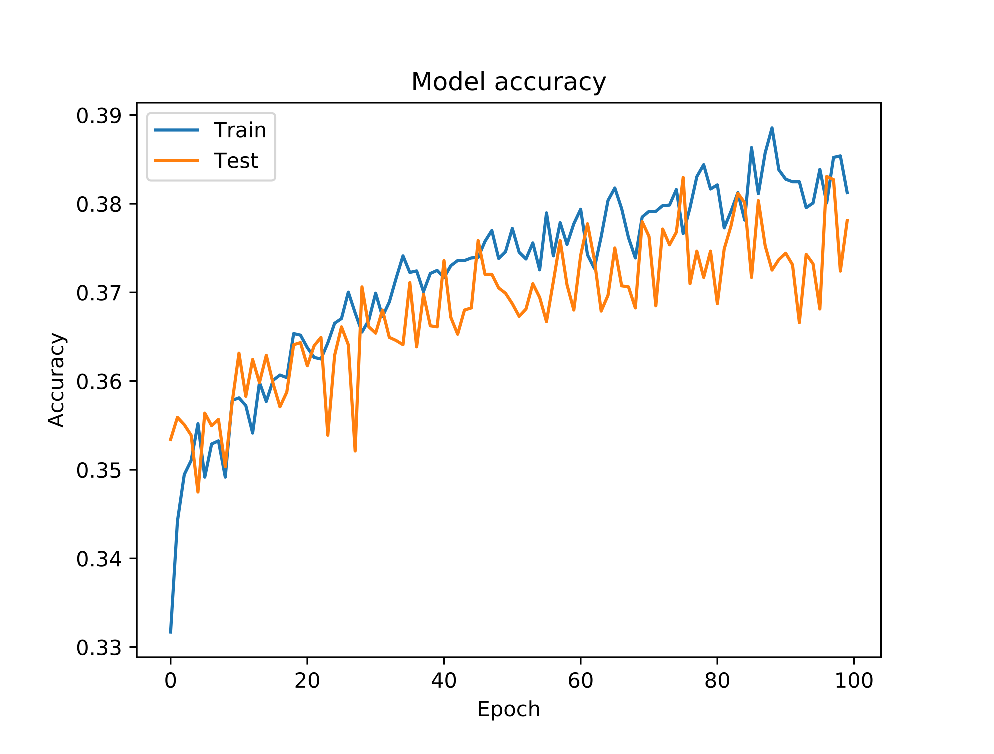
\includegraphics[height=2.5in]{vancouver-final.eps}
    \caption{Accuracy after epochs, with dropout layers. (Vancouver)}\label{van-final}
\end{figure}


\begin{figure}
    \centering
    \includegraphics[width=\textwidth]{cities.png}
    \caption{Classification accuracy in 5 cities}\label{cities}
\end{figure}


%%%%%%%%%%%% Section %%%%%%%%%%%%%%
\section{Conclusion}
In this project, we have successfully predicted the trend of some meteorological features using time-series model with decent confidence interval. The model extends the historical by 50\% from 6 years to 9 years, which provides useful data for related research and give people a clear image of how climate will change in the following years. Also, using a simple DNN model we are able to predict weather 5 days later with at least 50\% accuracy simply using temperature, humidity, pressure and wind data which are easy to measure. In the future, by adding more features such as climate type and using shift windows, we look forward to further increase the model accuracy so the prediction result may even have practical use in people's daily lives.

\begin{thebibliography}{8}
    \bibitem{abrahamsen2018machine}
    Erik Abrahamsen, Ole~Magnus Brastein, and Bernt Lie.
    \newblock Machine learning in python for weather forecast based on freely
    available weather data.
    \newblock In {\em Proceedings of The 59th Conference on Simulation and
    Modeling (SIMS 59), 26-28 September 2018, Oslo Metropolitan University,
    Norway}, number 153, pages 169--176. Link{\"o}ping University Electronic
    Press, 2018.
    
    \bibitem{holmstrom2016machine}
    Mark Holmstrom, Dylan Liu, and Christopher Vo.
    \newblock Machine learning applied to weather forecasting, 2016.

    \bibitem{liu2014deep}
    James~NK Liu, Yanxing Hu, Jane~Jia You, and Pak~Wai Chan.
    \newblock Deep neural network based feature representation for weather
    forecasting.
    \newblock In {\em Proceedings on the International Conference on Artificial
    Intelligence (ICAI)}, page~1. The Steering Committee of The World Congress in
    Computer Science, 2014.

    \bibitem{arxivadhi}
    Adhikari, R., \& Agrawal, R. K. (2013). An introductory study on time series modeling and forecasting. arXiv preprint arXiv:1302.6613

    \bibitem{boxcali}
    Box, G. E. P., \& Jenkins, G. M. (1970). Time Series Analysis Forecasting and Control/'Holden Day, San Francisco, California.

    \bibitem{zhangneur}
    Zhang, G. P. (2003). Time series forecasting using a hybrid ARIMA and neural network model. Neurocomputing, 50, 159-175.
\end{thebibliography}

\end{document}